\documentclass[../main/main.tex]{subfiles}


\begin{document}

\section{April 25th, 2019}
\subsection{Review of Multiway Cut Problem}
We are given an undirected graph $G=(V,E)$ with edge costs $c_e\ge 0$ for all $e\in E$. We also have $k$ distinguished vertices $s_1, s_2, \ldots,s_k$. \\

Our goal is to partition the set of vertices into sets $C_i$ such that $s_i \in  C_i$ for all $i$ and such that the cost of  \[
	F=\bigcup\limits_{i} \delta(C_i)
\] is minimum. In other words, we are trying to minimize the cost of the edges that cross the cuts.

This can be formulated as an ILP: 
\begin{itemize}
	\item For each vertex $u\in V$, introduce variable $x_u^i$ defined by: \[
	x^i_u=\begin{cases}
		1\quad\text{if $u$ is assigned to $C_i$}\\
		0\quad\text{otherwise}
	\end{cases}
	.\] 
\item For each edge $e\in E$, introduce variables $z_e^i$ which is defined by: \[
z_e^i=\begin{cases}
	1\quad\text{if $e\in \delta(C_i)$}\\
	0\quad\text{otherwise}
\end{cases}
.\] 
\item ILP: \[
		\min_e c_e\left( \frac{1}{2}\sum_i z_e^i \right) 
\] Subject to: \[
\sum_i x^i_u = 1
\] \[
z^i_e \ge x^i_u-x^i_v
\] \[
z^i_e\ge x^i_v - x^i_u
\] for all edges $e=(u,v)$, with connectivity and integer constraints: \[
x^i_{s_i}=1
\] \[
x^i_u \in \{0,1\} 
.\] 
\item For the LP relaxation, we have: \[
x_u^i \ge 0
.\] 
\end{itemize}
\subsection{LP Relaxation for the Multiway Cut Problem}
Think of $x_u$ as a point in $ k$ dimensions: \[
	x_u=(x_u^1, x_u^2,\ldots,x_u^k)
.\] For $k=3$ we can think as the following diagram:
\begin{figure}[h!]
	\centering
	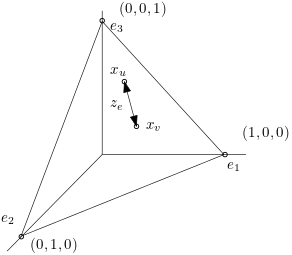
\includegraphics[width=0.5\textwidth]{4-25-k3}
	\label{fig:4-25-k3}
\end{figure}
\begin{remark}
Note that $x_{s_1}=(1,0,0), x_{s_2}=(0,1,0)$, i.e. \[
	x_{s_i}=e_i
.\] This means that $x_u$ is on the hyperplane going through $e_i$. In addition, note that the $x_u$ for the ILP lie on $e_i$.
\end{remark}

Define the simplex in $k$ dimension as: \[
\Delta_k= \{x\in R^{k}:\ \sum_i x^i=1\} 
.\] Note that: \[
\sum_i z^i_e = sum_i |x_u^i-x_v^i|
\] \[
\|x_u-x_v\|_1
,\] which is the $L_1$ distance between $x_u$ and $x_v$.\\

We can rewrite the relaxed LP as:
\[
	\min \frac{1}{2}\sum_{e=(u,v)} c_e \|x_u-x_v\|
\] subject to: \[
x_u\in \Delta_k
\] \[
x_{s_i}=e_i .\] 

In other words, we have to map the vertices the interior of this triangle, with cost being the weighted sum of the endpoints. This is called the \vocab{fractional multiway cut} 
\begin{figure}[h!]
	\centering
	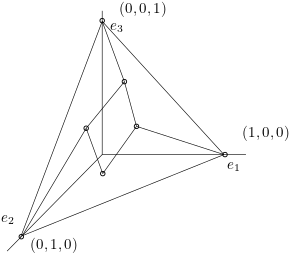
\includegraphics[width=0.5\textwidth]{4-25-k3-2}
	\caption{Fractional Mutiway Cut}
	\label{fig:4-25-k3-2}
\end{figure}

\begin{remark}
	Although this does not look like an LP, since it is the same as the LP, we can solve this in polynomial time.
\end{remark}

Now we will convert this back into a feasible solution through randomized rounding.

\subsection{Randomized Rounding}
The deterministic approach would be to take each vertex and map it to its nearest corner. However, there isn't much analysis to prove its factor. As such we will take a randomized approach.\\

If we call the ``ball distance'' as half the $L_1$ distance, the maximum ball distance between any two vertices is 1 (if they are at the corners).  Define $B(i_i,r)$ be the set of vertices $u$ such that: \[
		\frac{1}{2}\|e_i -x_u\|\le r
	.\] Note that all vertices are within ball distance $1$ from $s_i$, that is $B(e_i,1)=V$. (note that we use  $e_i$ and $s_i$ interchangeably.
\\

\begin{algo} 
	\begin{itemize}
		\item Solve LP optimally
	\item Select $r\in (0,1)$ uniformly at random
\item Assign vertices within $B(s_i,r)$ to $C_i$
\end{itemize}
\end{algo}
\begin{remark}
	The above algorithm has the following issues: 
	\begin{enumerate}
		\item Some vertices are not within ball-distance $r$ from any corner.
		\item Some vertices for which there is a conflict, where it is being assigned to multiple corners.
	\end{enumerate}
\end{remark}
\begin{algo}
	\begin{itemize}
		\item Select $r\in (0,1)$ uniformly at random.
		\item Select a random permutation $\Pi$ of $\{1,2,\ldots,k\} $ 
		\item Examine the vertices in the order given by the permutation $\Pi$.
		\item For index  $\Pi(i)$, assign all vertices not assigned so far in $B(s_{\Pi(i)},r)$ to $C_{\Pi(i)}$
		\item At the end of the order (i.e. when considering  $S_{\Pi(i)}$), assign all vertices not yet assigned to  $C_{\Pi(k)}$.
	\end{itemize}

\end{algo}
\begin{remark}
	Note that both issues with the previous algorithms are solved, as each vertex is given a chance to grab vertices, and all vertices are assigned.
\end{remark}
\subsection{Analysis of Randomized Rounding Algorithm}
To analyze this algorithm, we need to find the probability that  edge $e=(u,v)$ makes a contribution to the cost, i.e. $u$ and $v$ are assigned to different corner (if they are assigned to the same, then they would not make a contribution).\\

First assume that the probability that we separate $u$ and $v$ is $\frac{1}{2}\|x_u-x_v\|$. If we can show this, then the expected cost of the multiway cut will be as good as the fractional multiway cut. (which is not possible). As such, to have a approximation factor of $1.5$, we would like to show that the probability is at most $\frac{3}{4}\|x_u-x_v\|$, as: \[
	\text{Expected Cost} = \sum_{e=(u,v)} \frac{3}{4}c_e \|x_u-x_v\|=\frac{3}{2}\sum_{e=(u,v)} \frac{1}{2} \|x_u-x_v\|
.\] This is where we are headed. \\

(reworded) Recall that:  \[
	OPT \ge  \frac{1}{2}\sum_{e=(u,v)} c_e \|x_u-x_v\|
\] where $x_u$ and $x_v$ correspond to vertices $u,v $ respectively in the optimal LP solution. Suppose we can show that the probability that $u$ and $v$ are assigned to different $C_i$'s is $\le \frac{3}{4}\|x_u-x_v\|$, then the expected solution found has cost:  \[
\le \sum_{e=(u,v)}\frac{3}{4}c_e \|x_u-x_v\|=\frac{3}{2}\sum_{e=(u,v)}\frac{1}{2}\|x_u-x_v\|\le \frac{3}{2}OPT
.\] We will show that this is the case.


\end{document}

